\documentclass[
a4paper,
oneside,
10pt,
fleqn,
headsepline,
toc=listofnumbered, 
bibliography=totocnumbered]{scrartcl}

% deutsche Trennmuster etc.
\usepackage[T1]{fontenc}
\usepackage[utf8]{inputenc}
\usepackage[english, ngerman]{babel} % \selectlanguage{english} if  needed
\usepackage{lmodern} % use modern latin fonts

% Custom commands
\newcommand{\AUTHOR}{Michael Wieland}
\newcommand{\SECONDAUTHOR}{Fabian Hauser}
\newcommand{\INSTITUTE}{Hochschule für Technik Rapperswil}

% Jede Überschrift 1 auf neuer Seite
\let\stdsection\section
\renewcommand\section{\clearpage\stdsection}

% Multiple Authors
\usepackage{authblk}

% Include external pdf
\usepackage{pdfpages}

% Layout / Seitenränder
\usepackage{geometry}

% Inhaltsverzeichnis
\usepackage{makeidx} 
\makeindex

\usepackage{url}
\usepackage[pdfborder={0 0 0}]{hyperref}
\usepackage[all]{hypcap}
\usepackage{hyperxmp} % for license metadata

% Mathematik
\usepackage{amsmath}
\usepackage{amssymb}
\usepackage{amsfonts}
\usepackage{enumitem}

% Images
\usepackage{graphicx}
\graphicspath{{images/}} % default paths

% Boxes
\usepackage{fancybox}

%Tables
\usepackage{tabu}
\usepackage{booktabs} % toprule, midrule, bottomrule
\usepackage{array} % for matrix tables

% Multi Columns
\usepackage{multicol}

% Header and footer
\usepackage{scrlayer-scrpage}
\setkomafont{pagehead}{\normalfont}
\setkomafont{pagefoot}{\normalfont}
\automark*{section}
\clearpairofpagestyles
\ihead{\headmark}
\ohead{\TITLE}
\cfoot{\pagemark}

% Pseudocode
\usepackage{algorithm}
\usepackage{algorithmic}

% Code Listings
\usepackage{listings}
\usepackage{color}
\usepackage{beramono}

\definecolor{DarkPurple}{rgb}{0.4, 0.1, 0.4}
\definecolor{DarkCyan}{rgb}{0.0, 0.5, 0.4}
\definecolor{LightLime}{rgb}{0.3, 0.5, 0.4}
\definecolor{Blue}{rgb}{0.0, 0.0, 1.0}

\lstdefinestyle{eclipse-style}{
	language=Java,  
	columns=flexible,
	showstringspaces=false,     
	basicstyle=\footnotesize\ttfamily, 
	keywordstyle=\bfseries\color{DarkPurple},
	commentstyle=\color{LightLime},
	stringstyle=\color{Blue}, 
	escapeinside={£}{£}, % latex scope within code      
	morekeywords={length},
	numbers=left,
	numberstyle=\tiny\color{black},
	frame=single,
}
\lstset{style=eclipse-style}


% Theorems \begin{mytheo}{title}{label}
\usepackage{tcolorbox}
\tcbuselibrary{theorems}
\newtcbtheorem[number within=section]{definiton}{Definition}%
{fonttitle=\bfseries}{def}
\newtcbtheorem[number within=section]{remember}{Merke}%
{fonttitle=\bfseries}{rem}
\newtcbtheorem[number within=section]{hint}{Hinweis}%
{fonttitle=\bfseries}{hnt}

% Dokumentinformationen
\newcommand{\SUBJECT}{Report}
\newcommand{\TITLE}{Cloud Infrastructre Lab 2}

\begin{document}
	
% Front page
\title{\TITLE}
\subject{\SUBJECT}
\author{\SECONDAUTHOR}
\author{\AUTHOR}
\affil{\INSTITUTE}
\date{\today}
\maketitle

% Table of contents
\tableofcontents


% 06.10.2016, 23:55, as PDF to beat.stettler@ins.hsr.ch

%TODO Hostname pro Stock? i.O??? -> ??Um was ging's da schon wieder genau??

\section{Aufgabenstellung}
\subsection{Einleitung}
Gemäss der Aufgabenstellung

\begin{quotation}
	The fictional company BetaHouse Inc. is specialized in the high-frequency trading sector. In this exercise you will design the LAN part of the network, based on customer specifications. Part two will focus on the WAN integration with several remote locations throughout Switzerland (10+).
	
	Start with analyzing and characterizing the desired goals. Then go ahead with a logical network design. Based on that define the physical network. Document, review and change if needed until you get a satisfying solution. 
	
	\textbf{It’s important to describe your design decisions in your documentation.}
\end{quotation}

\subsection{Angaben zur Firma}

\begin{description}
	\item[Firmenname] BetaHouse Inc.
	\item[Niederlassungen] 10+, verbunden über WAN
\end{description}

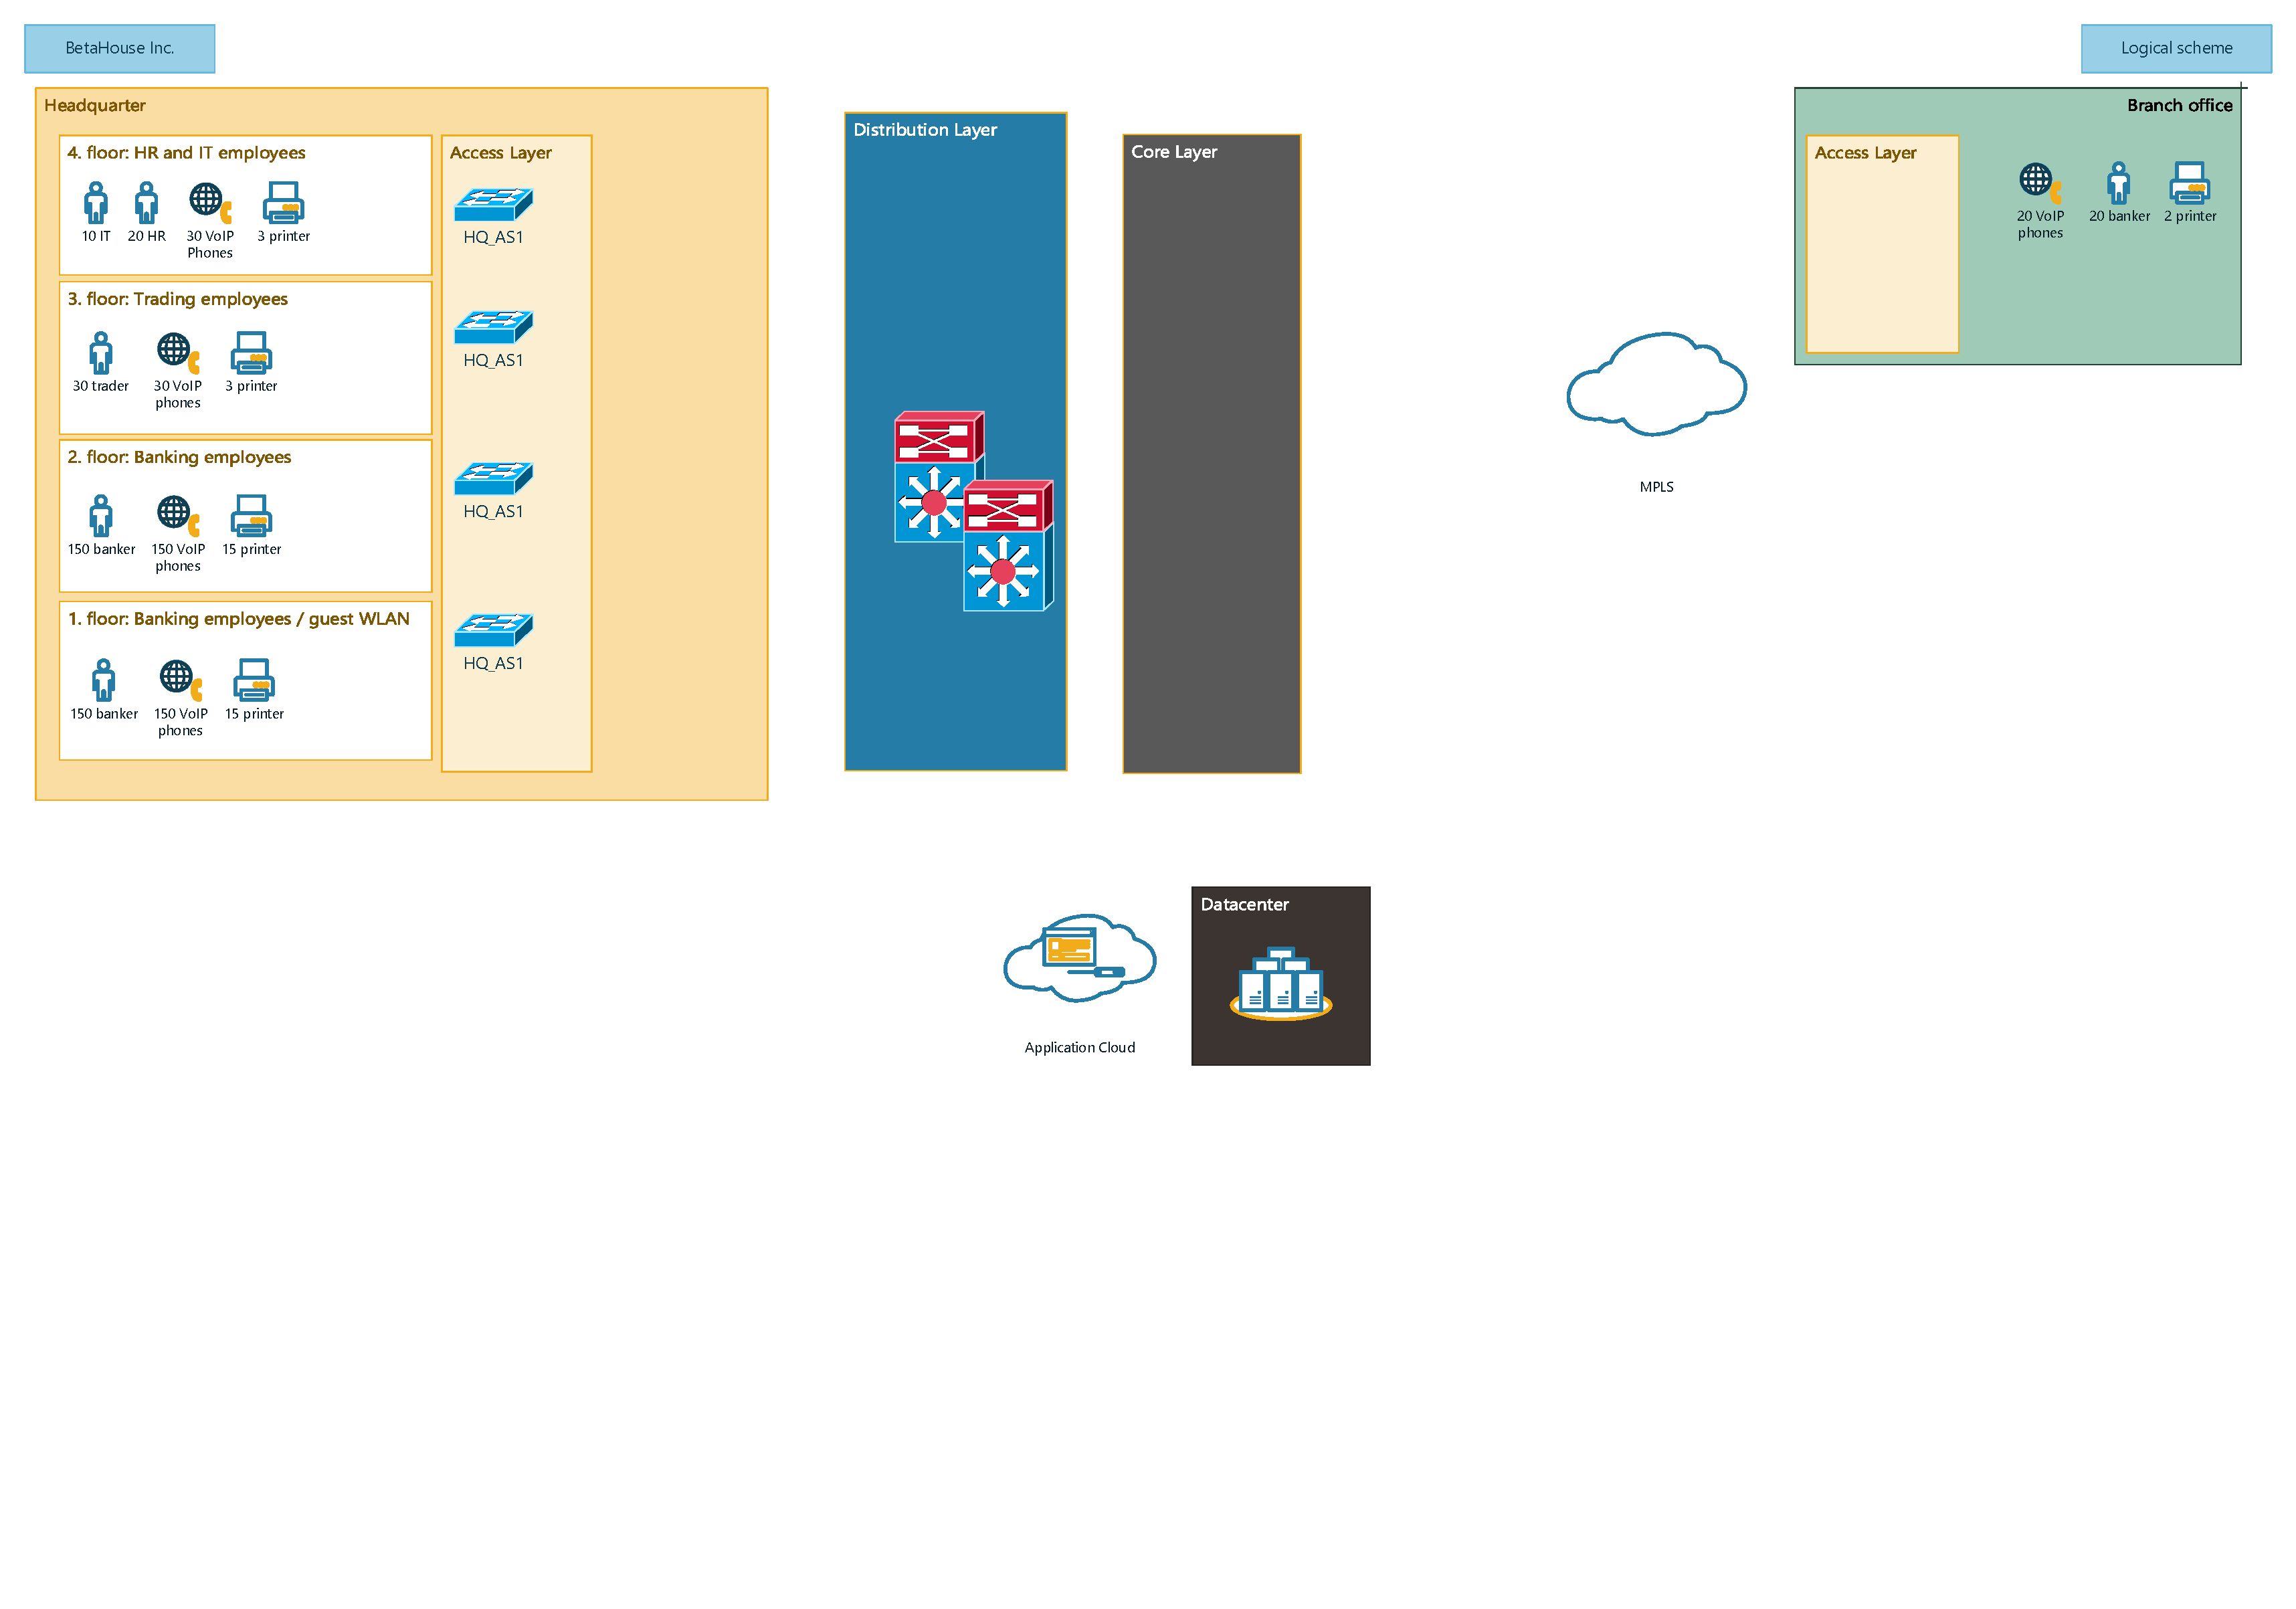
\includepdf[pages={1},landscape=true]{appendix/schemes/lan_logical.pdf}

\subsection{Vorgehen}
\begin{enumerate}
	\item Analyse der Kundenansprüche
	\item Designentscheidungen ausformulieren
	\item Aufbau des Campus LAN Design
	\item Aufbau des Adressierungs- \& Namensschema
	\item Analysieren Nutzung von Cloud Diensten
\end{enumerate}

\section{Design Headquarter}

\subsection{Kundenansprüche an das Netzwerk}

\subsubsection{Ansprüche Verfügbarkeit / Redundanz }
Da die Firma im Highspeed-Finanztrading arbeitet, ist eine zuverlässige Anbindung in und an die Firmeninfrastruktur essenziell. Besonders kommt dies bei der Trading-Abteilung zum tragen: Diese muss mit sehr grossen Beträgen in kurzer Zeit, ohne Unterbrüche handeln können. Deshalb sollte die Trading-Abteilung zusätzlich Redundant angeschlossen werden.

Grundsätzlich sind für die meisten Mitarbeiter eine Verfügbarkeit von ca. 99.99\% ausreichend, für die Trading-Abteilung sollte eine Verfügbarkeit von 99.999\% angestrebt werden.

Um diese Zahlen zu erreichen, müssen nahezu alle Geräte redundant ausgelegt sein (eine Doppelredundanz wird angestrebt; eine Dreifachredundanz würden Komplexität und Kosten zu stark erhöhen). Zudem müssen in der IT-Abteilung Strikte Verfahren festgelegt werden, welche die Konfiguration des Netzwerkes nur noch nach dem Vieraugenprinzip erlaubt. Damit wird die Fehlerwahrscheinlichkeit gesenkt.

\subsubsection{Datenfluss Netzwerk}

Der meiste Datenfluss im Netzwerk wird wohl von den Tradern ausgehen, da diese immer über aktuelle Ereignisse informiert sein müssen sowie häufig und viele Trading-Aktionen auslösen. Die anderen Abteilungen haben einen geringen bis mittleren Bedarf an Internet und internen Daten, sowie Anspruch an eine latenzarme Telefonielösung.

\paragraph{Datacenter}
Das Datacenter hat einen, durch die zentrale Funktion bedingten, höheren Netzwerk- und Redundanzbedarf. Das Datacenter stellt zudem Internetdienste (wie E-Mail und Webseite) sowie Terminal- und Telefonieserver im internen Netz für das Headquarter und die Branches zur Verfügung, und bedarf deshalb ein sehr Ausfallsicheres Netzwerk.

\paragraph{Aussenstandorte}

Die Aussenstandorte, welche über die MPLS-Cloud angeschlossen sind, benötigen einen stabile und performante Anbindung an das Datacenter, da die Mitarbeiter in erster Linie auf den Terminal-Servern und internen Cloud-Diensten arbeiten.

\subsubsection{Application QoS Ansprüche}

Der Latenzzeit bei BetaHouse Inc. ist insbesondere bei den Highspeed-Tradern sowie der Telefonie Beachtung zu schenken. Beim Highspeed-Trading kann die Konkurrenz schon nach wenigen Milisekunden einen Vorteil erwirtschaften; dies kann zu grossen Verlusten führen.

Bei der Telefonie ist es wichtig, dass die Latenzzeit unter 200ms, wenn möglich aber unter 100ms Ende-zu-Ende-Latenz liegen soll.

Zum sicherstellen der obenstehenden Geschwindigkeiten muss auf allen Routern ein QoS auf das Trading-Netzwerk sowie auf SIP/RTP bzw. SIPS/RTPS eingerichtet werden.


\paragraph{Firmenwachstum}
Bei den Schätzungen der Firmengrösse sind wir von einem Wachstum von $10\%$ pro Jahr qua Mitarbeiterzahl bzw. benötigten Geräten ausgegangen. Dies bedeutet auf eine 5-Jahres-Frist ein Wachstum von ca. $160\%$. 

\subsection{Campus LAN Design}

\subsubsection{Physische Netzwerkkarte}
Da Geschwindigkeit eine Kernanforderung in dem Trading Geschäft ist, haben wir im gesamten Netzwerk Gigabit Verbindungen aufgezogen. Im Core setzen zusätzlich auf Glasfasern.

\subsubsection{Logische Netzwerkkarte}
Das gesamte Netzwerk ist auf strikt nach den empfohlenen drei Ebenen ''Access'', ''Distribution'' und ''Core'' designed. Wir verwenden durchgehend Layer 3 Switches, damit wir komplett auf STP verzichten können. Spanning Tree wird in Computernetzen dieser Grössenordnung nicht empfohlen, da sie eine grosse Konvergenz aufweisen. VLAN's werden nur bis zu den Access Switches zur Trennung von VoIP Phones und Workstation verwendet. 

\subsection{WAN Network Design}

Bei den WAN-Netzwerken ist es für diesen Kunden essenziell, dass eine schnelle und stabile Anbindung an das Headquarter existiert, da die Mitarbeiter jeweils auf den Terminal-Servern im Datacenter arbeiten. Zudem soll es einfach möglich sein, neue Standorte hinzuzufügen.

Any-to-Any Konnektivität zum Senken der Latenzzeiten wäre zudem wünschenswert.

Ein kosteneffizienter, schneller und latenzarmer Ansatz wäre es daher, sich über einen Provider mittels Redundant angelegtem MPLS-Backbone zu verbinden. Mit dem Serviceprovider kann ein passendes SLA für die benötigten Verfügbarkeitszeiten ausgehandelt werden. So sollte das Netzwerk mindestens 99.99\% der Zeit voll funktionsfähig sein.

\subsection{Adressierungs- \& Namensschema}

Die IP-Adressierung wird optimiert auf Wachstumsmöglichkeiten und schnelles Routing über mehrere Standorte (mittels einfachem Zusammenfassen von Routen an den gleichen Standort.)

\subsubsection{Namensschema}

Die Netzwerkgeräte werden jeweils nach dem Standorttyp, falls vorhanden der Gebäudenummer, dem Gerätetyp und einer aufsteigenden Nummer (ohne führenden Nullen) benannt:

\lstinline|<Standort<Nummer>>_<Geraetetyp><Geraetenummer>|

\begin{table}[h]
	\centering
	\begin{tabu}{l l}
		\toprule
		Geräteort/Typ & Bezeichnung \\
		\midrule
		Headquarter & \lstinline|HQ|\\
		Standort / Branch & \lstinline|BRx| \\
		\midrule
		Access Switch & \lstinline|ASx|\\
		Distribution Switch & \lstinline|DSx|\\
		Core Switch & \lstinline|CSx|\\
		MPLS CE Router & \lstinline|CE|\\
		Firewall & \lstinline|FWx| \\
		Access Point & \lstinline|APx| \\
		ISP-Router & \lstinline|ISPx| \\
		\bottomrule
	\end{tabu}
	\label{tbl:nameing_scheme}
	\caption{Namensschema Netzwerkgeräte}
\end{table}

Beispiele: HQ\_AS3, BR3\_AS1

\subsubsection{VLAN}
Die VLANs werden intern in den Access-Switches verwendet, um die Port-Gerät Zuordnung festzulegen und einen entsprechenden virtuellen Routing-Port anzulegen. Die VLANs haben keinen Einfluss auf den weiteren Netzwerk-Pfad (Dieser wird auf Layer 3 behandelt, siehe Netzwerk-Diagramm)

\begin{table}[h]
	\centering
	\begin{tabu}{l l}
		\toprule
		Abteilung & Netzbereich \\
		\midrule
		IT & \lstinline|VLAN0001|\\
		Trading & \lstinline|VLAN0002| \\
		Banking & \lstinline|VLAN0003|\\
		HR & \lstinline|VLAN0004|\\
		Gäste & \lstinline|VLAN0005|\\
		(Datacenter \& Routing) & \lstinline|VLAN0006|\\
		(VoIP) & \lstinline|VLAN0250|\\
		\bottomrule
	\end{tabu}
	\label{tbl:vlans}
	\caption{VLAN-Abteilung-Zuordnung}
\end{table}


\subsubsection{IPv4}
Die internen IPv4 Adressen werden gemäss folgendem Schema aufgebaut: 

 \lstinline|10.<Standort>.<Abteilung>.0/24|
 
 Das Basisnetz ist 10.0.0.0/8. Für die Links werden je /30 Netze beginnend bei 10.0.0.0/30 erstellt.
 
\begin{table}[h]
	\centering
  \begin{tabu}{l l}
  	\toprule
  	Abteilung & Netzbereich \\
  	\midrule
  	IT & \lstinline|10.x.1.|\\
  	Trading & \lstinline|10.x.2.| \\
  	Banking & \lstinline|10.x.3.|\\
  	HR & \lstinline|10.x.4.|\\
 	Gäste & \lstinline|10.x.5.|\\
 	(Datacenter \& Routing) & \lstinline|10.x.200.|\\
 	(VoIP) & \lstinline|10.x.250.|\\
 	\bottomrule
  \end{tabu}
  \label{tbl:abteilung_ipv4_adressblock}
  \caption{Abteilung IPv4-Adressblock}
\end{table}

\begin{table}[h]
	\centering
	\begin{tabu}{l l}
		\toprule
		Standort & Netzbereich \\
		\midrule
		Links & \lstinline|10.0.0.0/30 .. 10.0.0.254/30| \\
		0. Floor & \lstinline|10.1.| \\
		1. Floor & \lstinline|10.2.| \\
		2. Floor & \lstinline|10.3.| \\
		3. Floor & \lstinline|10.4.| \\
		4. Floor & \lstinline|10.5.| \\
		Branch 1 & \lstinline|10.11.| \\
		Branch 2 & \lstinline|10.12.| \\
		Branch 3 & \lstinline|10.13.| \\
		Datacenter & \lstinline|10.200.| \\
		Datacenter DMZ & \lstinline|10.224.| \\
		\bottomrule
	\end{tabu}
	\caption{Standorte IPv4-Adressblock}
\end{table}

\subsubsection{IPv6}

Die internen IPv6 Adressen werden gemäss folgendem Schema aufgebaut: 

\lstinline|<Provider-Prefix>:<Standort><Abteilung>:<autoconf-eui-64>|

\begin{table}[h]
	\centering
	\begin{tabu}{l l}
		\toprule 
		Abteilung & Netzbereich \\
		\midrule
		IT & \lstinline|01|\\
		Trading & \lstinline|02| \\
		Banking & \lstinline|03|\\
		HR & \lstinline|04|\\
		Gäste & \lstinline|05|\\
		(Datacenter \& Routing) & \lstinline|C8|\\
		(VoIP) & \lstinline|FA|\\
		\bottomrule
	\end{tabu}
	  \label{tbl:abteilung_ipv6_adressblock}
	\caption{Abteilung IPv6-Adressblock}
\end{table}

\begin{table}[h]
	\centering
	\begin{tabu}{l l}
		\toprule
		Standort & Netzbereich \\
		\midrule
		Links & \lstinline|00| \\
		0. Floor & \lstinline|01| \\
		1. Floor & \lstinline|02| \\
		2. Floor & \lstinline|03| \\
		3. Floor & \lstinline|04| \\
		4. Floor & \lstinline|05| \\
		Branch 1 & \lstinline|0B| \\
		Branch 2 & \lstinline|0C| \\
		Branch 3 & \lstinline|0D| \\
		Datacenter & \lstinline|C8| \\
		\bottomrule
	\end{tabu}
	\caption{Standorte IPv6-Adressblock}
\end{table}
\clearpage

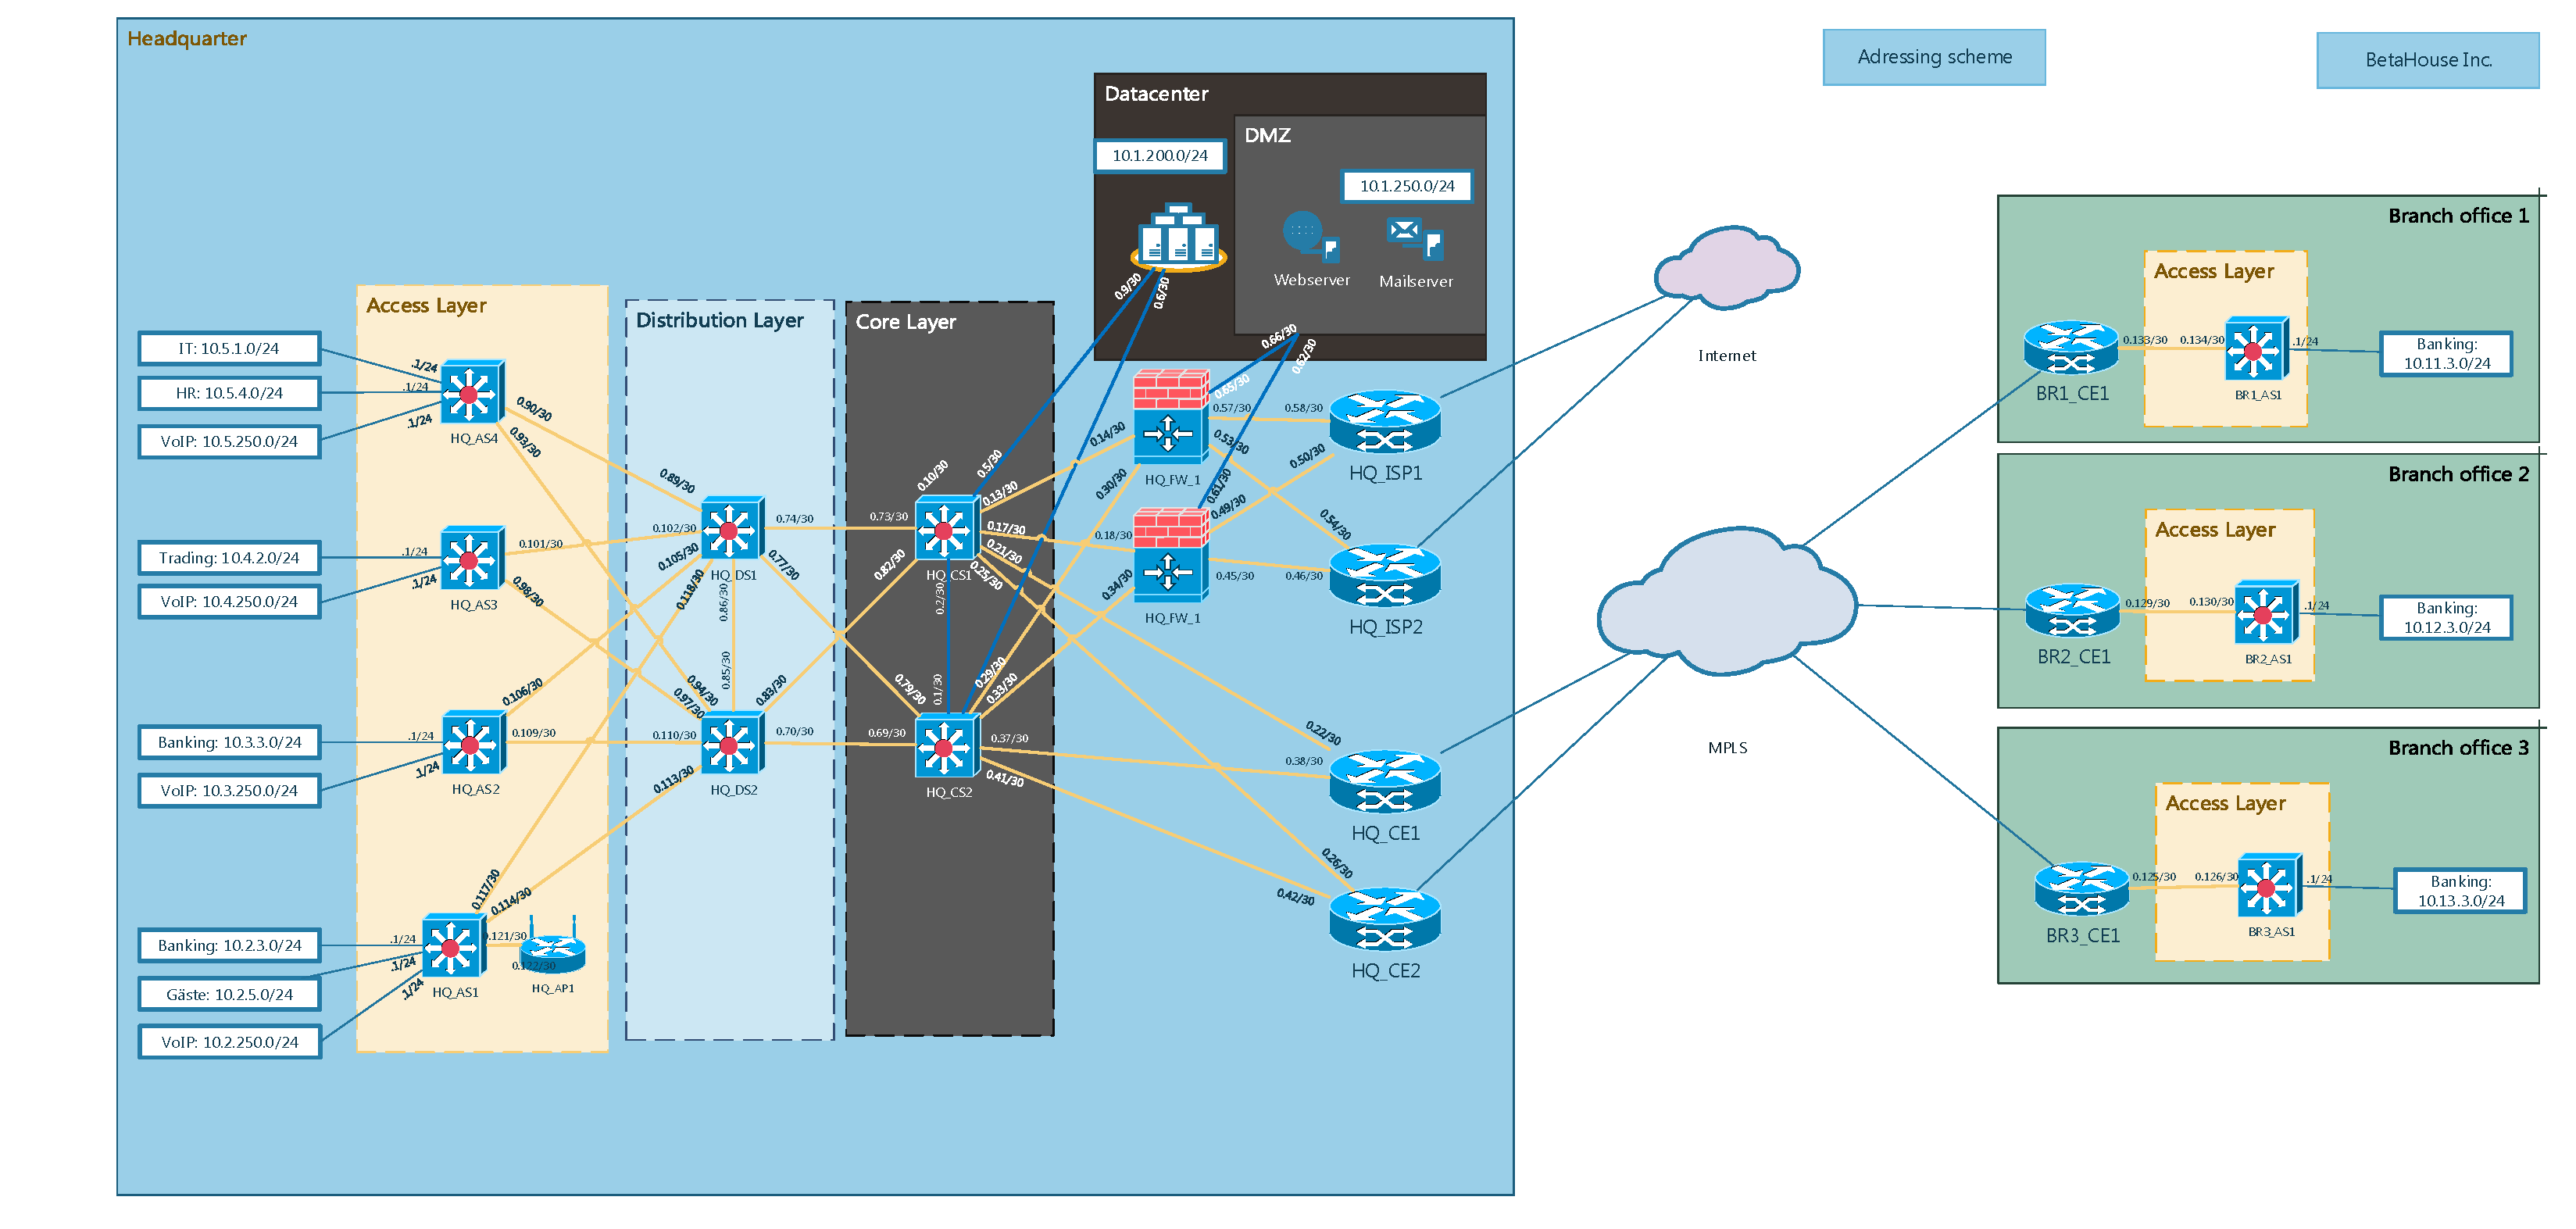
\includepdf[pages={1},landscape=true]{appendix/schemes/addressing.pdf}

\subsection{Benötigte Komponenten}
\subsubsection{Access Ports}
Minimal werden für das Netzwerk folgen Anzahl Access Ports benötigt. 
\begin{table}[h]
	\centering
	\begin{tabu} to \linewidth {l l l l l}
		\toprule
		Ort & Abteilung & Anz. Mitarbeiter & Anz. Drucker & Benötigte Access Ports \\
		\midrule
		HQ 1. Stock & Banking und Gäste & 150 & 15 & $150 + 15 + 1 = 166$ \\
		HQ 2. Stock & Banking & 150 & 15 & $150 + 15 = 165$ \\
		HQ 3. Stock & Trading & 30 & 3 & $2 \cdot 30 + 3 = 63$ \\
		HQ 4. Stock & IT und HR & $10 + 20 = 30$ & 3 & $30 + 3 = 33$\\
		Branch  & Banking & 20 & 2 & $20 + 2 = 22$\\
		\bottomrule 
	\end{tabu}
	\label{tbl:require_access_ports}
	\caption{Benötigte Access Ports}
\end{table}

\subsubsection{Switches}
Wir setzen im gesamten Netzwerk Cisco Layer 3 Switches mit je 48 Ports ein. Diese bieten die Möglichkeit sich als Stack zu organisieren. Jeder Stack wird über einen eigenen logischen Hostnamen angesprochen. Um die hohe Verfügbarkeit für die Trading Abteilung zu garantieren, schliessen wir die VoIP Phone an einem separaten Access Port an. Die 30 Trader werden zu jede 15 Personen an einen L3 Switch angeschlossen. So bleiben bei einem Ausfall immer die Hälfte der Trader voll operationsfähig. Um einen Ausfall möglichst zu vermeiden, sind alle Switches an einer USV angeschlossen. Da bei einem Ausfall der Switches in der Trading Abteilung grosse Kosten entstehen, hält sich die IT einen vorkonfigurierten Backup Switch in Ihrem Stockwerk. Damit kann im Notfall der Switch ohne grössere Zeitverluste ausgetauscht werden. Alle weiteren Abteilungen haben eine normale Wichtigkeit und werden gemäss ihrer Mitarbeiterzahl angeschlossen. Es wurde aber auch bei Ihnen ein Wachstum eingerechnet. Bei den VoIP Phones verwenden wir das Single Cable Design. Das bedeutet, dass die Workstations mit dem VoIP Phone verbunden und das Phone dann an den Access Switch angeschlossen wird. Die Daten werden mit tagged VLAN's getrennt. Aus der Tabelle \ref{tbl:require_access_ports} folgt, dass folgende Switches angeschafft werden müssen. 
\begin{table}[h]
	\centering
	\begin{tabu} to \linewidth {l l l X }
		\toprule 
		Bereich & Anzahl & Komponente & Hostname \\
		\midrule
		Guest WLAN & 1x & IEEE 802.11ac Access Point & HQ\_AP\_1 \\
		Banking HQ 1. floor & 4x & 48 Port Switch & HQ\_AS\_1 \\
		Banking HQ 2. floor & 4x & 48 Port Switch & HQ\_AS\_2 \\
		Trading HQ 3. floor & 2x & 48 Port Switch & HQ\_AS\_3 \\
		IT und HR HQ 4. floor & 1x & 48 Port Switch & HQ\_AS\_4 \\
		\midrule
		HQ Firewall & 2x & 8 Port Firewall & HQ\_FW\_x \\
		HQ MPLS Customer Edge Router & 2x & 8 Port Router & HQ\_CE\_x \\
		\midrule
		Branch 1 & 1x & 48 Port Switch & BR1\_AS\_1 \\
		Branch 2 & 1x & 48 Port Switch & BR2\_AS\_2 \\
		Branch 3 & 1x & 48 Port Switch & BR3\_AS\_3 \\
		BR MPLS Customer Edge Router & 3x & 8 Port Router & BR\_CE\_x \\
		\bottomrule 
	\end{tabu} 
	\caption{Benötigte Switches}
\end{table}

\subsection{Technologie \& Protokolle}
\subsubsection{Layer 2}
Wir verzichten auf STP, da wir für alle Bereiche eigene IP Subnetze verwenden. 

\subsubsection{MPLS}
Für die Anbindung der Branches haben wir uns für MPLS entschieden. Es bietet entscheidende Vorteile gegenüber einer Mitleitung oder einer Anbindung über Framerelay. So kann ein neuer Branch ohne grossen Aufwand in die MPLS Cloud eingefügt werden.

\subsubsection{Layer 3}
Für das Routing wird OSPF verwendet. Mehrere redundante Default-Gateways werden über HSRP ermöglicht.

\subsubsection{VoIP}
Grundsätzlich sind alle Workstations mit dem VoIP Phone an einem einzelnen Access Port angeschlossen. Der Verkehr wird über verschiedenen VLAN's strikt getrennt. Eine Ausnahme bildet einzig die Trading Abteilung, da diese auf eine hohe Verfügbarkeit der Telefone und Workstations angewiesen sind. Wir setzen für die Trading Abteilung deshalb auf separate Access Ports für die Workstation und das VoIP Telefon. Im Falle eines Ausfalls einer Komponente kann der Trade so trotzdem mit der zweiten weiterarbeiten, bis das Problem behoben ist.

\subsection{Security}

\subsubsection{Firewall}
Wir verwenden zwei Firewall die untereinander Load Balancing machen. Fällt eine aus, läuft kann der komplette Verkehr über die zweite Firewall nach wie vor ins Internet geroutet werden.

Die Firewalls stellen sicher, dass kein unerlaubter Verkehr aus dem Internet in die DMZ oder ein internes Netzwerk gelangt, und umgekehrt.

\subsubsection{WAN}
Die sichere Übertragung über das WAN wird über das MPLS-Netzwerk des Providers abgewickelt. Die Daten, welche über das MPLS-Netzwerk fliessen, sind nicht verschlüsselt, aber Physich und Logisch nur sehr schwer zugänglich. Sollte eine weitere Verschlüsselung gewünscht sein, müssten teure Hardware-Verschlüsselungsgeräte für jeden Standort angeschafft werden. Um dies entscheiden zu können, müsste die Architektur und Details der Applikationen bekannt sein.

\subsubsection{Interne Netzwerke}

Die internen Netzwerke sind von den Layer 3 Switches in einzelne IP-Subnetze und z.T. VLANs unterteilt. Dies stellt sicher, dass nur die Mitarbeiter der jeweiligen Abteilung in die betreffenden Netzwerke gelangen können.

Weitere Zugriffsberechtigungen können aus der IP-Adresse der Standorte und Abteilungen abgeleitet werden.

\subsubsection{DMZ}

Zur Trennung der internen Netzwerke und Internetdiensten wurde eine Demilitarisierte Zone (DMZ) für z.B. Webserver und Mailserver im Datacenter eingeplant.

\section{Organisation IT-Applikationen}

\subsection{Positionierung Applikationsserver}

Um eine ausfallsichere und schnelle Applikations-Infrastruktur zu ermöglichen, empfiehlt es sich, die Applikationsserver in erster Linie im Datacenter aufzustellen. Dies vereinfacht die Wartung und z.B. Anschluss an ein redundantes Netzwerk \& USV. Für einige Applikationen (Domain-Controller, VoIP) kann zur Verbesserung der Redundanz oder Latenzzeiten ein zusätzliches Gerät bei allen grösseren Aussenstandorten aufgestellt werden.

Für das High-Frequency-Trading ist eine kurze Leitung und Latenzfreie Verbindung zur Börse unerlässlich. Aus diesen Gründen könnte es sich lohnen, einen Rechenzentrumsplatz nahe der Börse zu mieten bzw. diese Geräte über einen nahe an der Börse gelegenen Standort zu betreiben.

\begin{table}[h]
	\centering
	\begin{tabu} to \linewidth {l l}
		\toprule
		Dienst & Standort(e) \\
		\midrule
		Domain Controller & Datacenter und Branches \\
		Mainfram for Banking-Application & Datacenter \\
		High Freuency Trading-Server & Datacenter oder Standort nahe Börse \\
		VoIP-Server & Datacenter sowie evtl. in Branches\\
		Backup Server & Datacenter \\
		\bottomrule
	\end{tabu} 
	\label{tbl:server_standorte}
	\caption{Serverstandorte Netzwerk}
\end{table}

\subsection{Cloud Dienste}

Für den zukünftigen Ausbau in der Benutzung von Cloud-Infrastrukturen würde es sich empfehlen, Standorte mit vielen Mitarbeitern neu direkt an das Internet anzubinden, anstatt wie bisher über das Headquarter

Dies hätte mehrere Vorteile; zum einen würde das WAN-Netzwerk weniger belastet, zum anderen sinken Latenzzeiten und steigt der mögliche Netzwerkdurchsatz. Ein weitere Nachteil wäre, dass neu an mehreren Standorten Firewall-Geräte notwendig sind. Dies steigert Kosten und Komplexität in der Konfiguration \& Routing.


\appendix

\section{Konfigurationen}
\label{appendix:configurations}

\subsection{BR1-R1}
\subsubsection{Running Configuration}
\lstinputlisting{appendix/config/br1-r1/br1-r1-config.txt}

\subsubsection{IP Interfaces}
\lstinputlisting{appendix/config/br1-r1/br1-r1-interface.txt}

\subsubsection{Interface Status}
\lstinputlisting{appendix/config/br1-r1/br1-r1-status.txt}

\subsubsection{Neighbors}
\lstinputlisting{appendix/config/br1-r1/br1-r1-neighbors.txt}

\subsection{BR2-R1}
\subsubsection{Running Configuration}
\lstinputlisting{appendix/config/br2-r1/br2-ri-config.txt}

\subsubsection{IP Interfaces}
\lstinputlisting{appendix/config/br2-r1/br2-ri-interface.txt}

\subsubsection{Interface Status}
\lstinputlisting{appendix/config/br2-r1/br2-ri-status.txt}

\subsubsection{Neighbors}
\lstinputlisting{appendix/config/br2-r1/br2-ri-neighbors.txt}

\subsection{BR2-S1}
\subsubsection{Running Configuration}
\lstinputlisting{appendix/config/br2-s1/br2-s1-config.txt}

\subsubsection{IP Interfaces}
\lstinputlisting{appendix/config/br2-s1/br2-s1-interface.txt}

\subsubsection{Interface Status}
\lstinputlisting{appendix/config/br2-s1/br2-s1-status.txt}

\subsubsection{Neighbors}
\lstinputlisting{appendix/config/br2-s1/br2-s1-neighbors.txt}

\subsection{CCNA-CCNP-FRSwitch}
\subsubsection{Running Configuration}
\lstinputlisting{appendix/config/framerelayswitch/framerelayswitch-config.txt}

\subsubsection{IP Interfaces}
\lstinputlisting{appendix/config/framerelayswitch/framerelayswitch-interface.txt}

\subsubsection{Interface Status}
\lstinputlisting{appendix/config/framerelayswitch/framerelayswitch-status.txt}

\subsubsection{Neighbors}
\lstinputlisting{appendix/config/framerelayswitch/framerelayswitch-neighbors.txt}

\subsection{HQ FrameRelay Router (HQ-FRR)}
\subsubsection{Running Configuration}
\lstinputlisting{appendix/config/hq-frr/hq-frr-config.txt}

\subsubsection{IP Interfaces}
\lstinputlisting{appendix/config/hq-frr/hq-frr-interface.txt}

\subsubsection{Interface Status}
\lstinputlisting{appendix/config/hq-frr/hq-frr-status.txt}

\subsubsection{Neighbors}
\lstinputlisting{appendix/config/hq-frr/hq-frr-neighbors.txt}

\subsection{HQ-IER1}
\subsubsection{Running Configuration}
\lstinputlisting{appendix/config/hq-ier1/hq-ier1-config.txt}

\subsubsection{IP Interfaces}
\lstinputlisting{appendix/config/hq-ier1/hq-ier1-interface.txt}

\subsubsection{Interface Status}
\lstinputlisting{appendix/config/hq-ier1/hq-ier1-status.txt}

\subsubsection{Neighbors}
\lstinputlisting{appendix/config/hq-ier1/hq-ier1-neighbors.txt}

\subsection{HQ-WER1}
\subsubsection{Running Configuration}
\lstinputlisting{appendix/config/hq-wer1/hq-wer1-config.txt}

\subsubsection{IP Interfaces}
\lstinputlisting{appendix/config/hq-wer1/hq-wer1-interface.txt}

\subsubsection{Interface Status}
\lstinputlisting{appendix/config/hq-wer1/hq-wer1-status.txt}

\subsubsection{Neighbors}
\lstinputlisting{appendix/config/hq-wer1/hq-wer1-neighbors.txt}

\subsection{HQ CS1}
\subsubsection{Running Configuration}
\lstinputlisting{appendix/config/hq-cs1/hq-cs1-config.txt}

\subsubsection{IP Interfaces}
\lstinputlisting{appendix/config/hq-cs1/hq-cs1-interface.txt}

\subsubsection{Interface Status}
\lstinputlisting{appendix/config/hq-cs1/hq-cs1-status.txt}

\subsubsection{Neighbors}
\lstinputlisting{appendix/config/hq-cs1/hq-cs1-neighbors.txt}

\subsection{HQ CS2}
\subsubsection{Running Configuration}
\lstinputlisting{appendix/config/hq-cs2/hq-cs2-config.txt}

\subsubsection{IP Interfaces}
\lstinputlisting{appendix/config/hq-cs2/hq-cs2-interface.txt}

\subsubsection{Interface Status}
\lstinputlisting{appendix/config/hq-cs2/hq-cs2-status.txt}

\subsubsection{Neighbors}
\lstinputlisting{appendix/config/hq-cs2/hq-cs2-neighbors.txt}

\subsection{HQ CS3}
\subsubsection{Running Configuration}
\lstinputlisting{appendix/config/hq-cs3/hq-cs3-config.txt}

\subsubsection{IP Interfaces}
\lstinputlisting{appendix/config/hq-cs3/hq-cs3-interface.txt}

\subsubsection{Interface Status}
\lstinputlisting{appendix/config/hq-cs3/hq-cs3-status.txt}

\subsubsection{Neighbors}
\lstinputlisting{appendix/config/hq-cs3/hq-cs3-neighbors.txt}

\subsection{HQ CS4}
\subsubsection{Running Configuration}
\lstinputlisting{appendix/config/hq-cs4/hq-cs4-config.txt}

\subsubsection{IP Interfaces}
\lstinputlisting{appendix/config/hq-cs4/hq-cs4-interface.txt}

\subsubsection{Interface Status}
\lstinputlisting{appendix/config/hq-cs4/hq-cs4-status.txt}

\subsubsection{Neighbors}
\lstinputlisting{appendix/config/hq-cs4/hq-cs4-neighbors.txt}

\subsection{HQ DS1}
\subsubsection{Running Configuration}
\lstinputlisting{appendix/config/hq-ds1/hq-ds1-config.txt}

\subsubsection{IP Interfaces}
\lstinputlisting{appendix/config/hq-ds1/hq-ds1-interface.txt}

\subsubsection{Interface Status}
\lstinputlisting{appendix/config/hq-ds1/hq-ds1-status.txt}

\subsubsection{Neighbors}
\lstinputlisting{appendix/config/hq-ds1/hq-ds1-neighbors.txt}

\subsection{HQ DS2}
\subsubsection{Running Configuration}
\lstinputlisting{appendix/config/hq-ds2/hq-ds2-config.txt}

\subsubsection{IP Interfaces}
\lstinputlisting{appendix/config/hq-ds2/hq-ds2-interface.txt}

\subsubsection{Interface Status}
\lstinputlisting{appendix/config/hq-ds2/hq-ds2-status.txt}

\subsubsection{Neighbors}
\lstinputlisting{appendix/config/hq-ds2/hq-ds2-neighbors.txt}

\subsection{HQ DS3}
\subsubsection{Running Configuration}
\lstinputlisting{appendix/config/hq-ds3/hq-ds3-config.txt}

\subsubsection{IP Interfaces}
\lstinputlisting{appendix/config/hq-ds3/hq-ds3-interface.txt}

\subsubsection{Interface Status}
\lstinputlisting{appendix/config/hq-ds3/hq-ds3-status.txt}

\subsubsection{Neighbors}
\lstinputlisting{appendix/config/hq-ds3/hq-ds3-neighbors.txt}


\section{Messungen}
\label{appendix:measures}
\subsection{Von X nach Y}
\lstinputlisting{appendix/config/br2-r1/br2-ri-config.txt}

% Code Listings
% \lstlistoflistings

% List of figures
% \listoffigures

% List of tables
% \listoftables

% Bibliography
% \bibliographystyle{plain} 
% \bibliography{literatur}

\end{document}
